% 原书 p.153–p.167（PDF p.161–p.175）
\section{辛同调（Symplectic Homology）}

% >>> p161
辛同调是一种用 Floer 理论研究刘维尔区域的方法，其中刘维尔区域在 3.2 节中定义。
本节中，我们将集中于图 6.4 左图所示的一类刘维尔区域
$W\subset(\C^n,\dd\lambda_{\mathrm{std}})$。回忆 $\partial W$ 是一个切触流形，其
切触结构由 $\xi=\ker(\lambda_{\mathrm{std}}|_{\partial W})$ 给出。

\begin{keytakeaways}
\begin{itemize}
  \item 几何图像：研究 $\C^n$ 中的刘维尔区域 $W$——用「指示函数」$\chi_W$ 作哈密顿
        函数，让它的哈密顿流在 $W$ 的边界上「捕捉」闭 Reeb 轨道。
  \item 数学工具：辛同调 $\mathrm{SH}_*^{(a,\infty)}(W)$ 定义为过滤哈密顿 Floer
        同调关于函数族的逆向极限；持续模语言把逆向极限与条形码联系起来。
  \item 关键结论：对 $(\C^n,\dd\lambda_{\mathrm{std}})$ 中的刘维尔区域，
        $\mathrm{SH}_*(W)$ 恒为零，但持续模 $\mathbb{V}_W$ 极不平凡
        （例 6.3.5）；对余盘丛 $D_g^*Q$，Viterbo 同构把辛同调等同于圈空间同调
        （定理 6.3.1）。
\end{itemize}
\end{keytakeaways}

\begin{figure}[htbp]
  \centering
  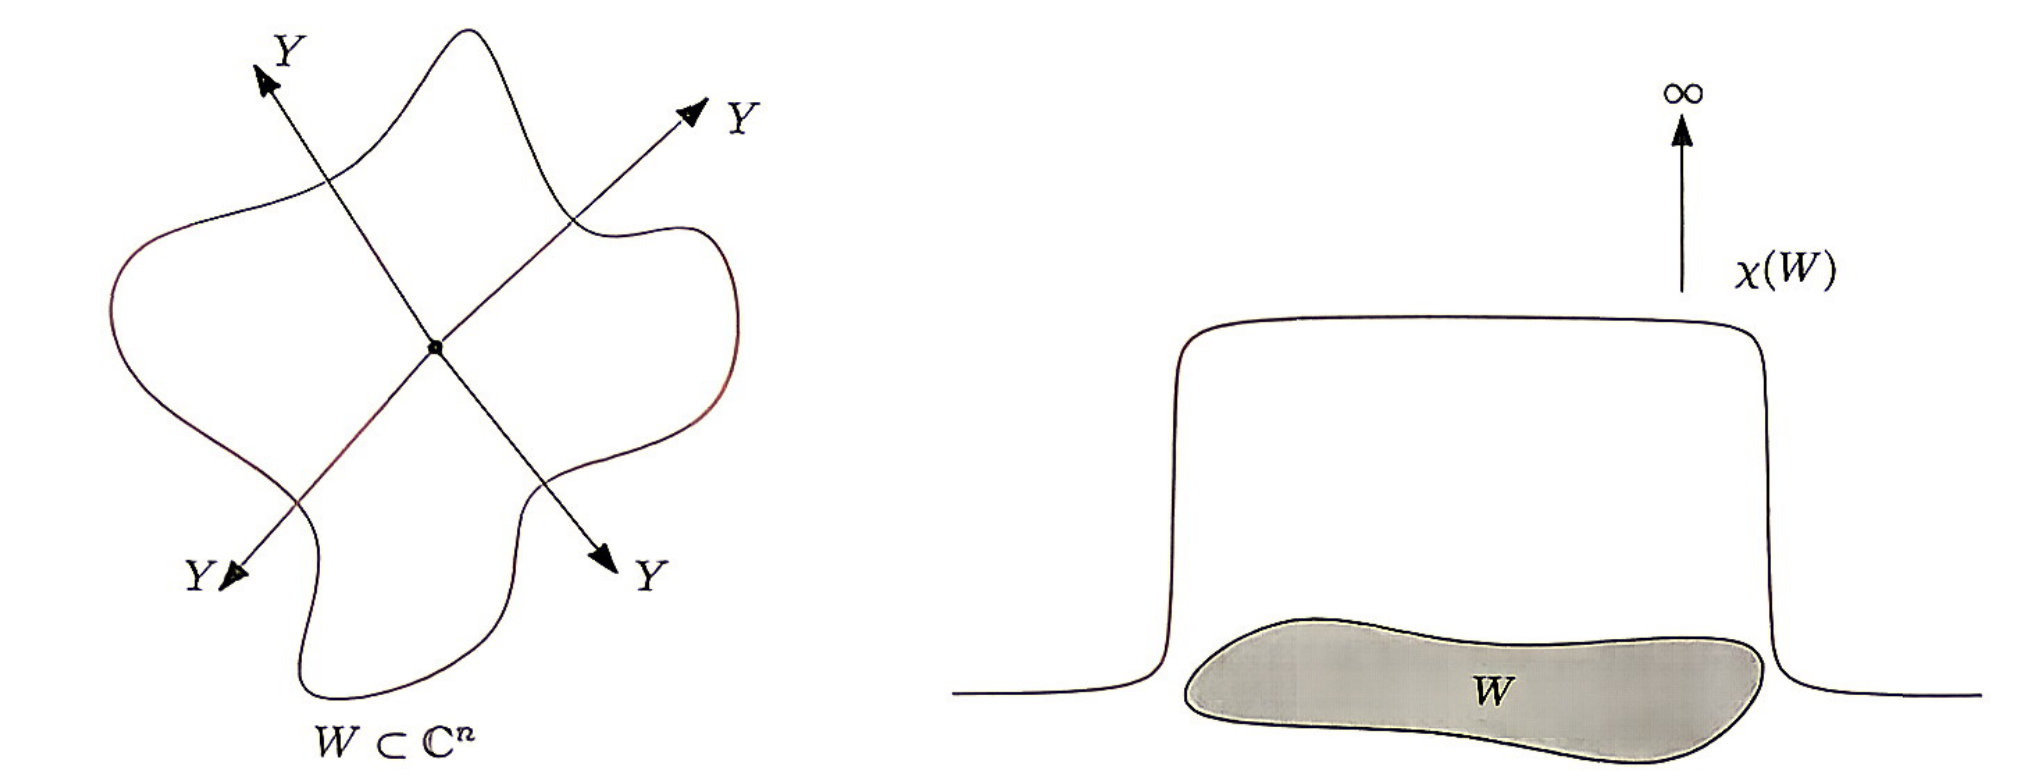
\includegraphics[width=0.92\linewidth]{figures/fig_p161_1.png}
  \caption*{图 6.4\quad 星形区域 $W\subset\C^n$ 与 $W$ 上的指示函数
    （原书 p.153, Figure 6.4；PDF p.161）}
\end{figure}

构造 $W$ 的辛同调的主要思路，是取「$W$ 的指示函数 $\chi_W$」作为哈密顿函数，使它
的哈密顿流捕捉到 $\partial W$ 上的一些切触几何动力学（更确切地说，Reeb 动力学）。
由于我们并不关心 Reeb 流的时间 1 映射，故允许哈密顿同痕流到 $t\to\infty$，这等价于
允许指示函数 $\chi_W$ 增长到无穷（见图 6.4 右图）。显然，就应用 5.4 节发展起来的
哈密顿 Floer 同调理论而言，这个指示函数 $\chi_W$ 是有问题的，因为它非常退化。稍后
我们将看到，如何通过选取一列逼近 $\chi_W$ 的函数来克服这一困难。

% >>> p162
对区域 $W$，为启动构造，我们将考虑一族「好的」刘维尔区域
$W\subset(\C^n,\dd\lambda_{\mathrm{std}})$：要求其中每一个的切触边界
$(\partial W,\ker(\lambda_{\mathrm{std}}|_{\partial W}))$（或简称 $\partial W$）满足
一个非退化性质。其\textbf{谱}（spectrum）定义如下：
\[
  \operatorname{Spec}\bigl(\partial W,\ker(\lambda_{\mathrm{std}}|_{\partial W})\bigr)
  :=\{\eta\in\R\mid \eta\ \text{是}\ \partial W\ \text{上某条闭 Reeb 轨道的周期}\}.
\]
若其切触边界的谱是 $\R$ 的离散子集，则称 $W$ 是\textbf{非退化刘维尔区域}。

\begin{wexam}{6.3.1}
  回忆四维辛椭球 $E(a,b)$ 在 (3.7) 中定义。则其切触边界 $\partial E(a,b)$ 非退化
  当且仅当 $a/b\notin\Q$。在这个非退化情形，$\partial E(a,b)$ 恰有两条素闭 Reeb
  轨道，它们的周期分别为 $a\pi$ 与 $b\pi$。\hfill$//$
\end{wexam}

为把 Floer 理论植入刘维尔区域 $W\subset\C^n$ 的研究，回忆 (3.10)：$\C^n$ 可以
作如下分解：
\begin{equation}\tag{6.7}
  \C^n=S(\partial W)\cup\{0\},
\end{equation}
其中 $S(\partial W)$ 是 $(\partial W,\ker(\lambda_{\mathrm{std}}|_{\partial W}))$ 的
辛化（见定义 3.2.1）。为简便，记 $\alpha=\lambda_{\mathrm{std}}|_{\partial W}$。
取坐标 $(r,p)$，把 $S(\partial W)$ 写成 $S(\partial W)=(0,\infty)\times\partial W$，
于是 $S(\partial W)$ 上的辛结构为 $\dd(r\alpha)$（cf.\ 定义 3.2.1 中的 (3.14) 与
练习 3.2.1）。特别地，$\partial W=\{r=1\}$，且
$W=\{0\}\cup((0,1]\times\partial W)=\{r\le 1\}$。

% [Tutor Note: 易错预警——这里的 $(r,p)$ 是辛化坐标：$r\in(0,\infty)$ 沿辛化方向，
% $p\in\partial W$；辛形式是 $\dd(r\alpha)=\dd r\wedge\alpha+r\,\dd\alpha$，
% 而不是 $\dd\alpha$ 的「齐次化」。注意 $r=1$ 给出边界 $\partial W$，$r\to0$
% 对应 $\C^n$ 的原点 $\{0\}$，故 $W=\{r\le1\}$ 是「星形」的。$\alpha$ 的限制
% 与 $\xi=\ker\alpha$ 的选取有关；改变 $\alpha$ 为 $e^f\alpha$ 会改变 $r$ 的
% 标度，从而改变 (6.8) 中作用量的具体表达式，但不变量的整体结构不变。]

\begin{wexam}{6.3.2}[承例 6.3.1]
  按定义，辛椭球 $E(a,b)$ 可显式地表示为
  \[
    E(a,b)=\left\{(z_1,z_2)\in\C^2\;\middle|\;
    \frac{|z_1|^2}{a}+\frac{|z_2|^2}{b}\le 1\right\}.
  \]
  于是，按本例正上方引入的记号，$W=E(a,b)$；并且在坐标变换
  \[
    (z_1,z_2)\mapsto\left(r=\frac{|z_1|^2}{a}+\frac{|z_2|^2}{b},\ 
    p=(\varphi_1,\varphi_2,\varphi_3)\right)
  \]
  之下（其中 $p=(\varphi_1,\varphi_2,\varphi_3)$ 是 $\C^2$ 中标准单位 3-球面的
  极坐标），有 $E(a,b)=\{r\le1\}$。\hfill$//$
\end{wexam}

% >>> p163
考虑 $\C^n$ 上不依赖于 $p$ 的哈密顿函数 $H(r,p)=h(r)$（见图 6.5）。人们或许会问
相应的哈密顿动力学行为如何。让我们计算其闭哈密顿轨道。按定义，
\begin{align*}
  -\dd h(r)&=-\dd H(r,p)=\omega_{(r,p)}\bigl(X_H(r,p),\,\cdot\,\bigr)\\
  &=(r\,\dd\alpha+\dd r\wedge\alpha)\bigl(X_H(r,p),\,\cdot\,\bigr),
\end{align*}
因为 $\omega=\dd(r\alpha)$。令 $X_H=A\partial_r+B$。这里 $\partial_r$ 沿辛化方向。
分量 $B$ 表示 $T\partial W$ 中的向量，故可写成 $B=C+f\cdot R_\alpha$，其中
$C\in\xi=\ker\alpha$，$f$ 是 $\partial W$ 上的函数。代入上式，得
\[
  -h'(r)\dd r=r\,\dd\alpha(C,\,\cdot\,)+A\alpha-f\cdot\dd r,
\]
这蕴含 $C=0$、$A=0$ 以及 $f=h'(r)$。因此
\[
  X_H(r,p)=h'(r)R_\alpha(p).
\]
由此我们断定：$\C^n$ 上哈密顿函数 $H(r,p)=h(r)$ 的一条闭哈密顿轨道满足下述两条
初等但重要的性质。
\begin{enumerate}[label=(\roman*)]
  \item 它是 $(\partial W,\ker\alpha)$ 上的一条闭 Reeb 轨道，周期为 $h'(r)$，
        其中 $r$ 满足 $h'(r)\in\operatorname{Spec}\bigl(\partial W,
        \ker(\lambda_{\mathrm{std}}|_{\partial W})\bigr)$。
  \item 它完全位于水平集 $\{r\}\times\partial W$ 中。
\end{enumerate}

\begin{figure}[htbp]
  \centering
  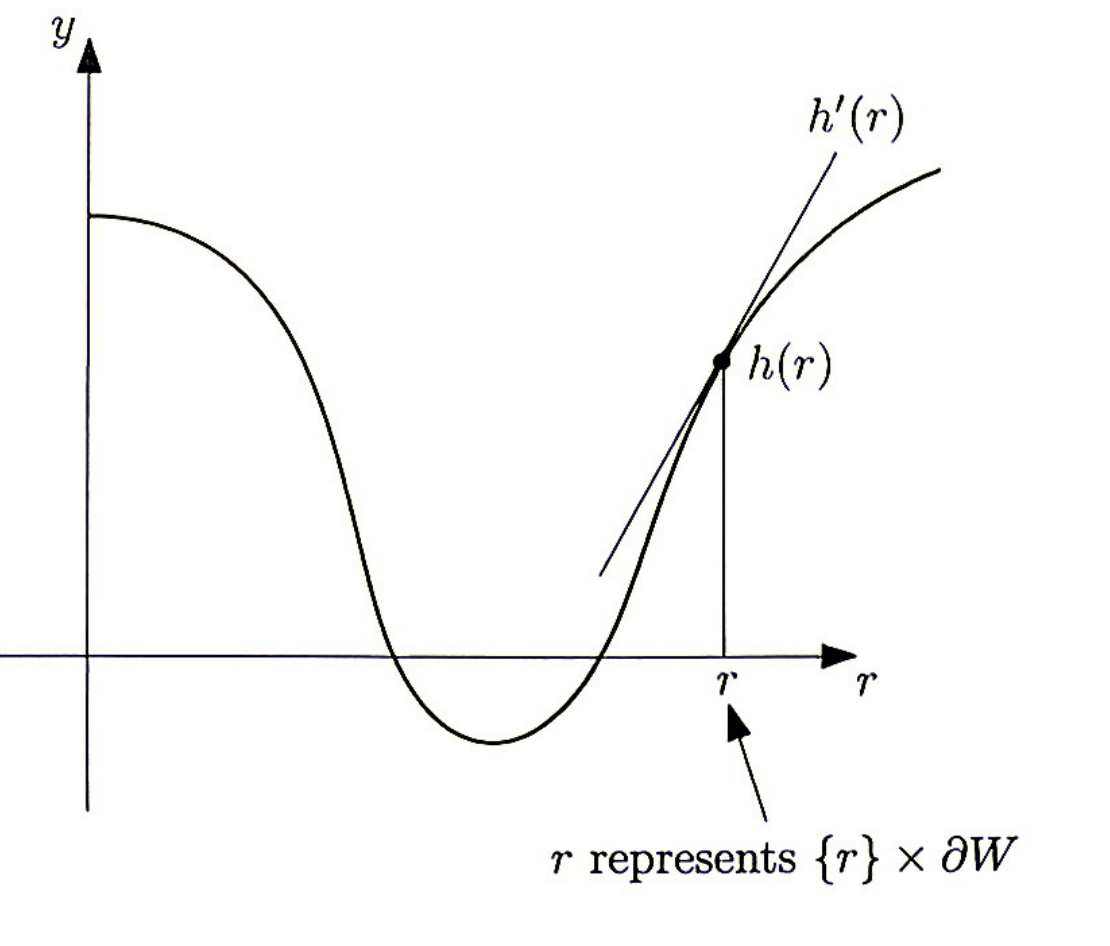
\includegraphics[width=0.47\linewidth]{figures/fig_p163_1.png}
  \caption*{图 6.5\quad $h(r)$ 与点 $r$ 处 $h'(r)$ 的图像
    （原书 p.155, Figure 6.5；PDF p.163）}
\end{figure}

固定这样一条闭哈密顿轨道 $x=x(t)$——把它看作 $\{r\}\times\partial W$ 上周期为
$h'(r)$ 的闭 Reeb 轨道。哈密顿 Floer 理论以 (5.17) 中定义的辛作用量泛函
$\mathcal{A}_H$ 为基础，把它作为圈空间 $\mathcal{L}M$ 上的「Morse 函数」。由于
$S(\partial W)$ 是恰当的，

% [Tutor Note: 易错预警——上述推导的关键是 $\iota_{X_H}\omega=-\dd H$ 的符号约定
% 与 $\omega=\dd(r\alpha)=\dd r\wedge\alpha+r\,\dd\alpha$ 的分解。逐项核对：
% $\iota_{A\partial_r}\omega=A\alpha$（因为 $\iota_{\partial_r}\dd r=1$、
% $\iota_{\partial_r}\dd\alpha=0$）；$\iota_B(\dd r\wedge\alpha)=-\alpha(B)\dd r$；
% 而 $\iota_B(r\,\dd\alpha)=r\,\dd\alpha(B,\cdot)$，且
% $\dd\alpha(R_\alpha,\cdot)=0$ 恰是 Reeb 向量的定义。比较 $\alpha$、$\dd r$、
% $\xi$ 三个分量即得 $A=0$、$f=h'(r)$、$C=0$。若符号约定相反（$\iota_{X_H}\omega=\dd H$），
% 则 $h$ 应换成 $-h$，向量场 $X_H=-h'(r)R_\alpha$。]

% >>> p164
对 (5.17) 中的第一项，由 Stokes 定理有
\[
  -\int_{D^2}w^*\omega=-\int_{S^1}x^*(r\alpha).
\]
由于闭哈密顿轨道 $x\subset\{r\}\times\partial W$，我们知道
\begin{equation}\tag{6.8}
  \mathcal{A}_H(x)
  =-r\cdot\alpha\bigl(h'(r)R_\alpha(p)\bigr)+h(x(t))
  =-r\cdot h'(r)+h(r).
\end{equation}
这一计算结果 $-r\cdot h'(r)+h(r)$ 有明显的几何意义。见图 6.6：轮廓曲线 $h(r)$ 在
$r_\ast$ 处切线的 $y$-截距为 $y=-r_\ast h'(r_\ast)+h(r_\ast)$。因此，对这一族特殊
的哈密顿函数，$\mathcal{A}_H(x)$ 就是该 $y$-截距。

\begin{figure}[htbp]
  \centering
  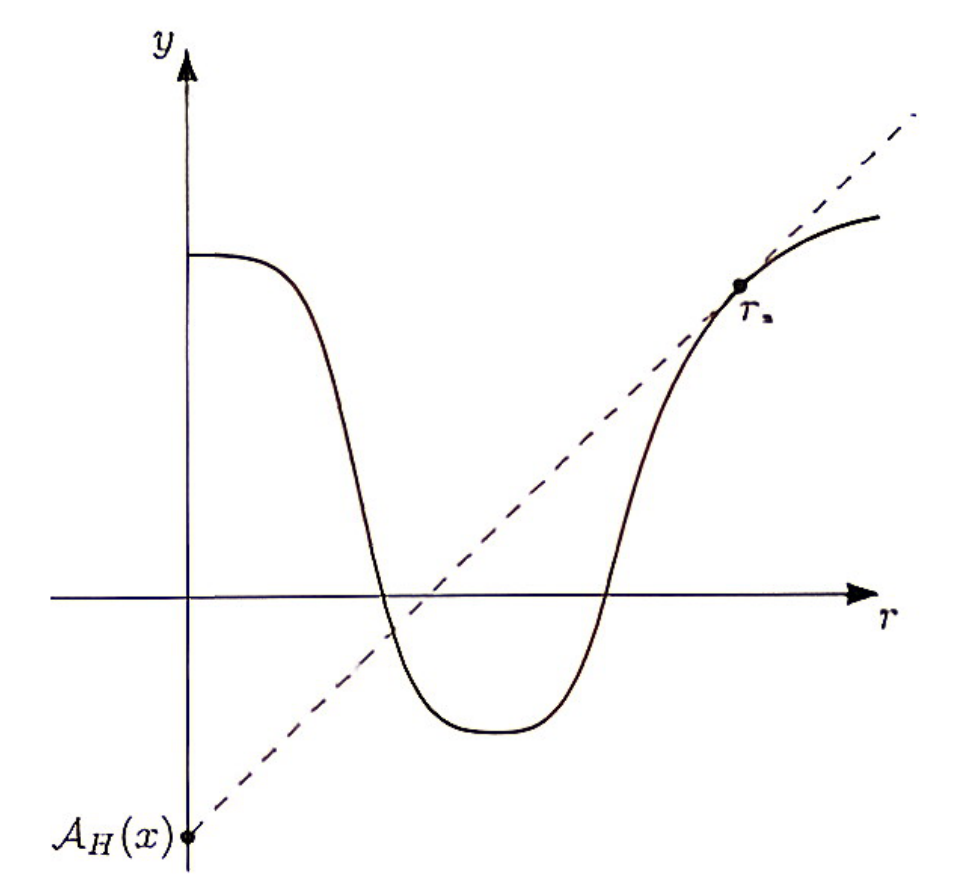
\includegraphics[width=0.52\linewidth]{figures/fig_p164_1.png}
  \caption*{图 6.6\quad $h(r)$ 与 $h'(r)$ 的图像（原书 p.156, Figure 6.6；PDF p.164）}
\end{figure}

\begin{wexam}{6.3.3}[承例 6.3.2]
  考虑四维椭球 $E(1,\pi)\subset\C^2$。由例 6.3.1 它是非退化的，且谱为
  \[
    \operatorname{Spec}\bigl(\partial E(1,\pi),
    \ker(\lambda_{\mathrm{std}}|_{\partial E(1,\pi)})\bigr)=\Z\cup\pi\Z.
  \]
  取 $\C^2$ 上如下形状的哈密顿函数 $H(r,p)=h(r)$：紧支撑于 $E(1,\pi)$ 的内部，
  且在 $E(1,\pi)$ 内部的大部分区域上是线性的。我们可以假设从某个小 $\varepsilon>0$
  出发、$r=1+\varepsilon$ 起恒有 $h(r)\equiv0$。再取 $\varepsilon$ 足够小，使得在
  线性部分上斜率落在下述窗口内：
  \[
    -4<\frac{-\pi}{1-\varepsilon}=h'(r)<-\pi.
  \]
  在 $r=0$ 处把 $h(r)$ 磨光，使得 $0$ 是 $h(r)$ 在 $0$ 的邻域内唯一的临界点。示意图
  见图 6.7 的左图。

  由上面的讨论，我们可以直接从图 6.7 的右图读出闭哈密顿轨道以及它们在
  $\mathcal{A}_H$ 下的作用量。具体地说，除了

% [Tutor Note: 易错预警——例 6.3.3 的斜率窗口
% $-4<-\pi/(1-\varepsilon)=h'(r)<-\pi$ 容易被误读为自相矛盾，其实因为
% $0<1-\varepsilon<1$，有 $\pi/(1-\varepsilon)>\pi$，故
% $-\pi/(1-\varepsilon)<-\pi$，右侧不等式自动成立；左侧不等式
% $-4<-\pi/(1-\varepsilon)$ 等价于 $\pi/(1-\varepsilon)<4$，即
% $\varepsilon<1-\pi/4\approx0.215$。所以只要 $\varepsilon$ 足够小（这已由
% 「$h$ 在 $r\ge1+\varepsilon$ 上为零、在线性部分斜率落入窗口」的选取保证），
% 整个连不等式是自洽的。核对时勿把 $-\pi/(1-\varepsilon)$ 看成比 $-\pi$ 更接近 $0$。]

% >>> p165
\begin{figure}[htbp]
  \centering
  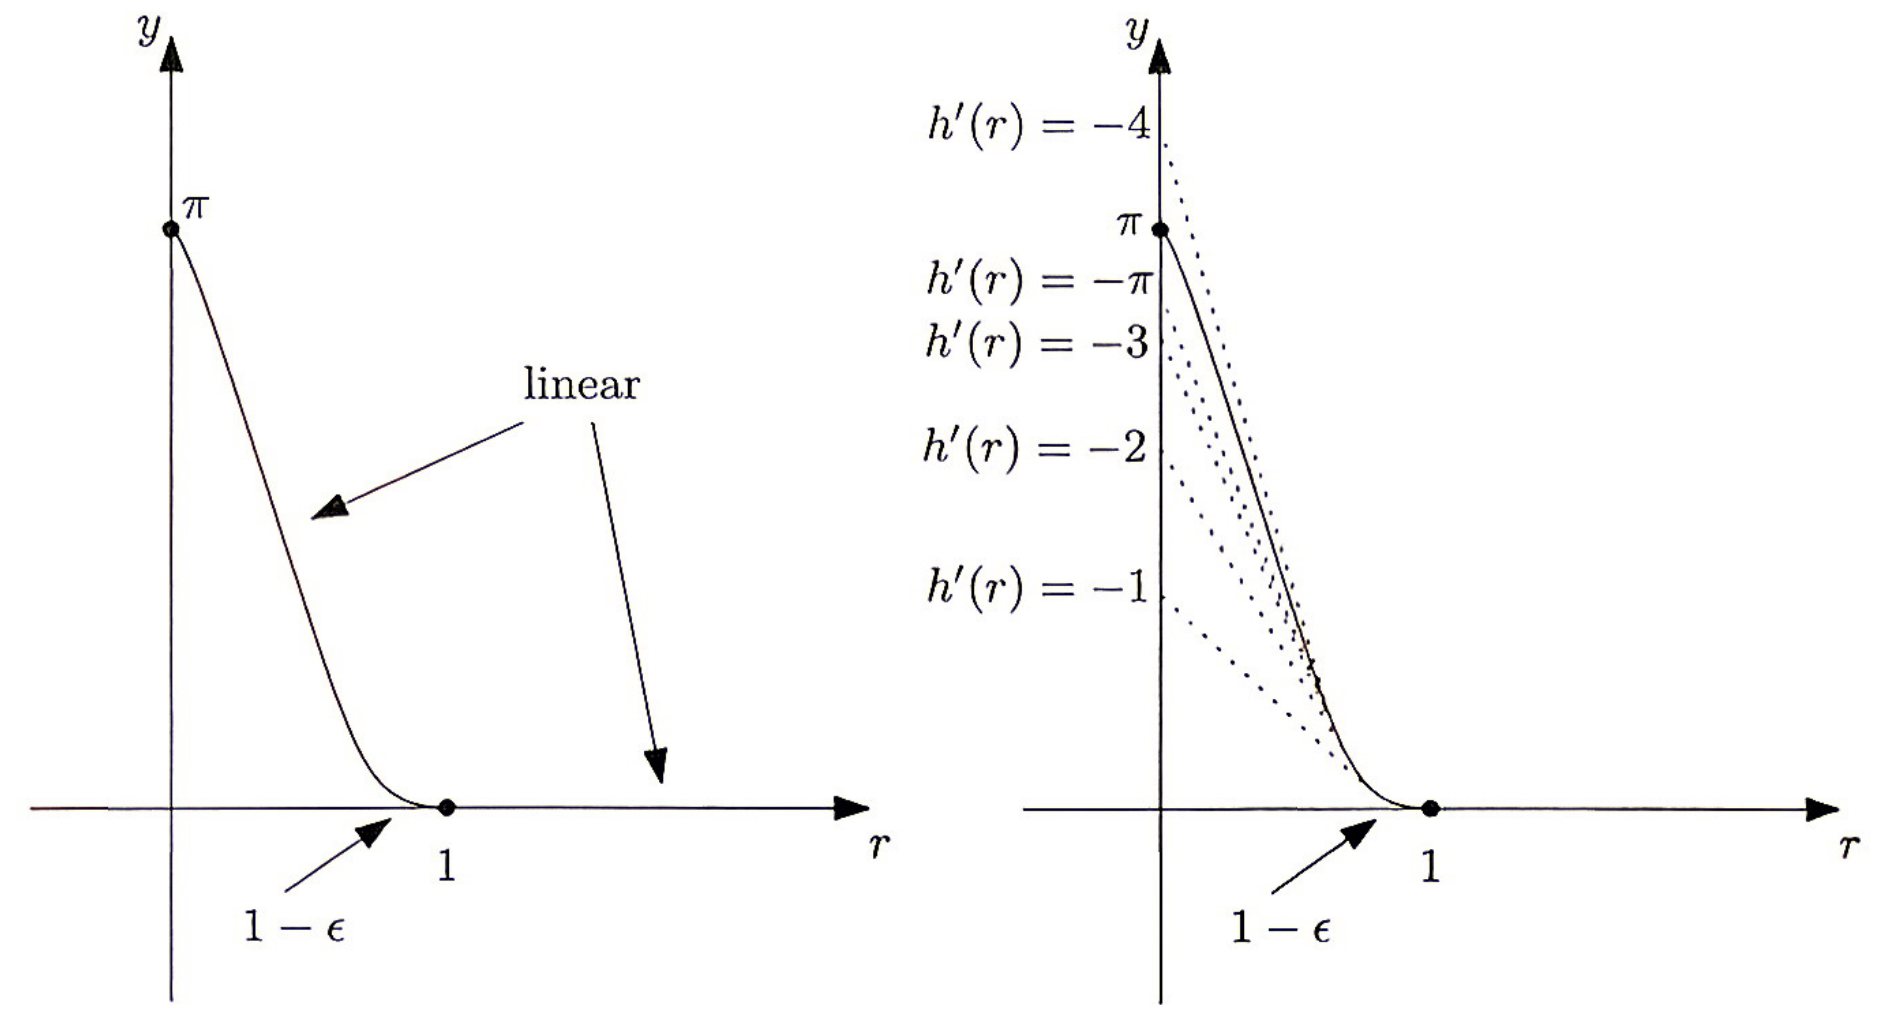
\includegraphics[width=0.9\linewidth]{figures/fig_p165_1.png}
  \caption*{图 6.7\quad $E(1,\pi)$ 上的 $h(r)$（原书 p.157, Figure 6.7；PDF p.165）}
\end{figure}

与 $0$ 处以及区域 $\{r\ge1+\varepsilon\}$ 中所有点所表示的常值闭哈密顿轨道不同，
其余的轨道来自 $(\partial E(1,\pi),\lambda_{\mathrm{std}}|_{\partial E(1,\pi)})$ 的
闭 Reeb 轨道，其周期为
\[
  h'(r)=k\quad\text{或}\quad h'(r)=l\pi,
  \qquad k,l\in\Z\setminus\{0\}.
\]
更准确地说，$k=-1,-2,-3$，$l=-1$。\hfill$//$
\end{wexam}

\begin{wrem}{6.3.1}
  (i) 一般说来，$h'(r)$ 与 $\mathcal{A}_H$ 的行为彼此独立。(ii) 注意：尽管
  $0\in\C^2$ 表示一条常值闭哈密顿轨道，但可以验证它是定义 5.4.1 意义下的非退化
  轨道。
\end{wrem}

为展示深刻的结果，让我们考虑另一个例子：在把轮廓函数 $h(r)$ 于所有「转折点」
（例如 $r=0.8$、$r=1$ 与 $r=2$）附近磨光之前，哈密顿函数 $H(r,p)=h(r)$ 如图 6.8
所示。

由与上面例 6.3.2 相同的讨论，存在闭哈密顿轨道 $x_1,x_3$ 出现在 $r=1$ 附近，
$x_2$ 出现在 $r=2$ 附近，且它们的作用量满足下述不等式
\begin{equation}\tag{6.9}
  \mathcal{A}_H(x_3)<\mathcal{A}_H(x_2)<\mathcal{A}_H(x_1).
\end{equation}
模仿 Morse 理论中「连接 $\Crit(F)$ 中两个不同点的负梯度流总使 Morse 函数 $F$ 的值
减小」（cf.\ 练习 5.1.1）这一事实，沿连接两条不同闭哈密顿轨道的负梯度流移动时，
辛作用量将会减小。特别地，不存在从 $x_3$ 到 $x_2$ 的 Floer 轨道（即满足方程
(5.21) 的轨道）。有趣的是，我们有下述断言，它排除了相反方向 Floer 轨道的存在。

% >>> p166
\whead{断言}{6.3.1}在图 6.8 所示的哈密顿动力学中，不存在从 $x_2$ 到 $x_3$ 的
Floer 轨道。

\begin{figure}[htbp]
  \centering
  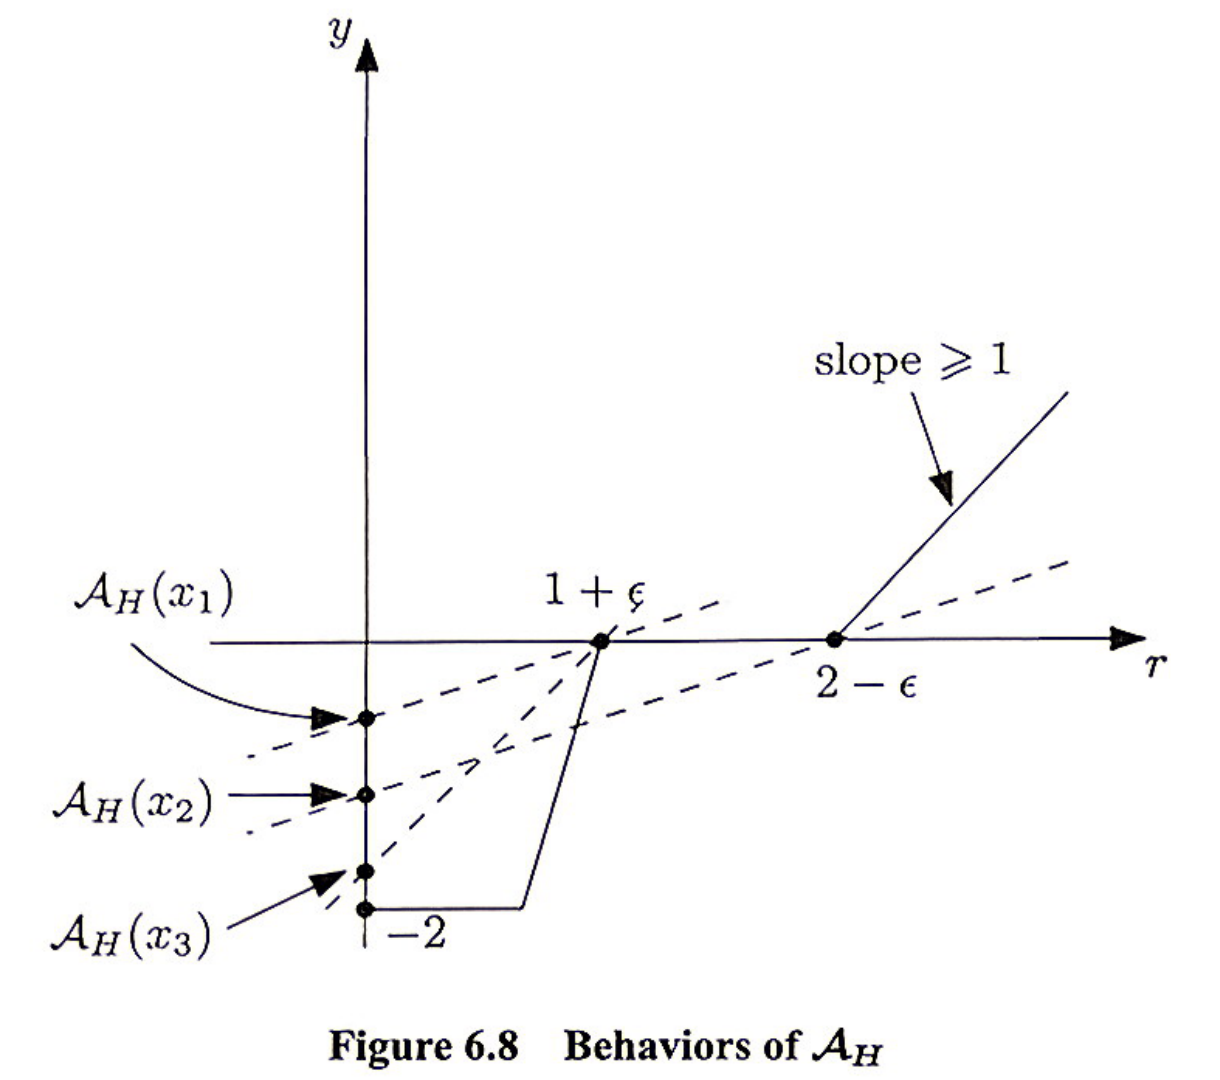
\includegraphics[width=0.58\linewidth]{figures/fig_p166_1.png}
  \caption*{图 6.8\quad $\mathcal{A}_H$ 的行为（原书 p.158, Figure 6.8；PDF p.166）}
\end{figure}

回忆：计数 Floer 轨道至关重要，因为它决定了 Floer 边界算子
$\partial_*\colon\mathrm{CF}_*(M,\omega,H,J)\to\mathrm{CF}_{*-1}(M,\omega,H,J)$。
因此，知道或界定（某些闭哈密顿轨道之间的）Floer 轨道的存在性，对于直接计算或估计
从相应哈密顿 Floer 同调中提取的某些不变量大有帮助。在许多情形（或许断言 6.3.1 所
提及的情形也是如此），5.5 节展示的指标也足以排除 Floer 轨道。这里我们只关注作用量，
并强调：断言 6.3.1 中的那些 Floer 轨道\emph{不能}仅通过考察 (6.9) 那样的作用量
关系来排除。

断言 6.3.1 的证明是一般结果命题 6.3.1 的直接推论，该命题专门适用于 $\C^n$ 中的
伪全纯曲线。这里，$\C^n$ 按 (6.7) 分解，其中大部分是辛化 $S(\partial W)$（对给定的
刘维尔区域 $W\subset(\C^n,\dd\lambda_{\mathrm{std}})$）。回忆 3.3 节中，对精心设计
的近复结构 $J$，我们研究了 $S(\partial W)$ 中的 $J$-全纯曲线。借用那里的策略（例如
(3.18)），我们将引入下述记号。

固定 3.3 节中的近复结构 $J$。给定辛作用量泛函 $\mathcal{A}_H$ 的一条负梯度流，
即映射 $u(s,t)\colon\R\times S^1\to(\C^n,\dd\lambda_{\mathrm{std}},J)$，由 (5.21)
它是扰动的 $J$-全纯柱面。在分解 (6.7) 之下，把它看作
\begin{equation}\tag{6.10}
  u(s,t)=\bigl(a(s,t),f(s,t)\bigr).
\end{equation}

% >>> p167
其中 $a(s,t)\colon\R\times S^1\to\R_{>0}$，$f(s,t)\colon\R\times S^1\to\partial W$。
于是 (5.21) 可写成
\begin{equation}\tag{6.11}
  \left(\frac{\partial a}{\partial s},\frac{\partial f}{\partial s}\right)
  +J(u(s,t))\left(\frac{\partial a}{\partial t},\frac{\partial f}{\partial t}\right)
  -J(u(s,t))h'(a(s,t))R_\alpha(f(s,t))=0.
\end{equation}
由于 $\partial_s f$ 落在切触流形 $\partial W$ 的切空间中，把它分解为
\[
  \frac{\partial f}{\partial s}
  =\alpha\left(\frac{\partial f}{\partial s}\right)R_\alpha
  +\pi_\xi\left(\frac{\partial f}{\partial s}\right),
\]
其中 $\pi_\xi$ 是到 $\partial W$ 上切触平面场的投影；对 $\partial_t f$ 类似。于是
(6.11) 改写为下述微分方程组：
\begin{equation}\tag{6.12}
  \begin{cases}
    \dfrac{\partial a}{\partial s}
    -\alpha\left(\dfrac{\partial f}{\partial t}\right)+h'(a(s,t))=0,\\[8pt]
    \alpha\left(\dfrac{\partial f}{\partial s}\right)
    +\dfrac{\partial a}{\partial t}=0,\\[8pt]
    \pi_\xi\left(\dfrac{\partial f}{\partial s}\right)
    +J(u(s,t))\pi_\xi\left(\dfrac{\partial f}{\partial t}\right)=0.
  \end{cases}
\end{equation}
这里有一个直接来自 (6.12) 的关键观察：对切触 1-形式
$\alpha(=\iota_{\lambda_{\mathrm{std}}}|_{\partial W})$，(6.10) 中的分量 $f$ 满足
$f^*\dd\alpha\ge0$。确实，

% [Tutor Note: 原文疑误——此处原文印作 $\alpha(=\iota_{\lambda_{\mathrm{std}}}
% |_{\partial W})$，其中记号 $\iota_{\lambda_{\mathrm{std}}}$ 无定义；结合本节前面
% 刚定义的 $\alpha=\lambda_{\mathrm{std}}|_{\partial W}$，此处的 $\iota$ 极可能是
% $\lambda$ 的排印之误。译文保留原文写法，已在 review_ch06.md 中记录，建议核对
% 原书（应为 $\alpha=\lambda_{\mathrm{std}}|_{\partial W}$）。]
\begin{align*}
  \dd\alpha\left(\frac{\partial f}{\partial s},\frac{\partial f}{\partial t}\right)
  &=\dd\alpha\left(\pi_\xi\left(\frac{\partial f}{\partial s}\right),
    \pi_\xi\left(\frac{\partial f}{\partial t}\right)\right)\\
  &=\dd\alpha|_\xi\left(-J\pi_\xi\left(\frac{\partial f}{\partial t}\right),
    \pi_\xi\left(\frac{\partial f}{\partial t}\right)\right)\\
  &=\dd\alpha|_\xi\left(\pi_\xi\left(\frac{\partial f}{\partial t}\right),
    J\pi_\xi\left(\frac{\partial f}{\partial t}\right)\right)\\
  &=g_J\left(\pi_\xi\left(\frac{\partial f}{\partial t}\right),
    \pi_\xi\left(\frac{\partial f}{\partial t}\right)\right)\ge0.
\end{align*}

% [Tutor Note: 易错预警——上述链中第三行的换序用到 $\dd\alpha$ 的反对称性：
% $\dd\alpha(-Ju,v)=\dd\alpha(v,Ju)$（删去负号），而第四行用 $g_J(\cdot,\cdot)
% :=\dd\alpha(\cdot,J\cdot)$ 的定义得到非负性。这里 $g_J$ 是把 $J$ 与 $\dd\alpha$
% 复合所得切触平面场 $\xi$ 上的度量。另注意 (6.12) 三条方程分别对应 (6.11) 的
% $\partial_r$ 分量、$\alpha$ 分量与 $\xi$ 分量；第三个方程即
% $\pi_\xi(\partial_s f)=-J\pi_\xi(\partial_t f)$，是把 $J$ 限制在 $\xi$ 上的
% 近复结构方程。]

这一观察是下述命题的关键步骤，该命题最终将用于证明断言 6.3.1。

\begin{wprop}{6.3.1}
  给定刘维尔区域 $W\subset(\C^n,\dd\lambda_{\mathrm{std}})$，设
  $u(s,t)\colon\R\times S^1\to\C^n$ 是（在分解 (6.7) 之下）由哈密顿函数
  $H(r,p)=h(r)$ 给出的 $\C^n$ 上哈密顿动力学的 Floer 轨道（即满足 (5.21)），
  其边界条件为
  \[
    \lim_{s\to-\infty}u(s,t)=(r_-,x_-(t))
    \quad\text{与}\quad
    \lim_{s\to+\infty}u(s,t)=(r_+,x_+(t)),
  \]
  其中 $x_-$ 与 $x_+$ 都是 $(\partial W,\ker(\lambda_{\mathrm{std}}|_{\partial W}))$
  的闭 Reeb 轨道，$r_-,r_+\in\R$。则我们有下述约束。
  \begin{enumerate}[label=(\roman*)]
    \item 若 $h''(r_-)>0$，则存在 $(s_\ast,t_\ast)\in\R\times S^1$ 使得
          $a(s_\ast,t_\ast)>r_-$，或者 $u(s,t)\equiv(r_-,x_-)$。
% >>> p168
    \item 若 $h''(r_+)<0$，则存在 $(s_\ast,t_\ast)\in\R\times S^1$ 使得
          $a(s_\ast,t_\ast)>r_+$，或者 $u(s,t)\equiv(r_+,x_+)$。
  \end{enumerate}
\end{wprop}

\begin{wproof}
  只需证明 (i)；把 $h$ 换成 $-h$，同样的论证即得 (ii)。假设 (i) 不成立，则对所有
  $(s,t)\in\R\times S^1$ 有 $a(s,t)\le r_-$。由于 $h''(r_-)>0$，可以假设存在
  $R_-\in\R$ 使得对任意 $(s,t)\in(-\infty,R_-)\times S^1$ 有
  $h''(a(s,t))\ge0$。不失一般性，设 $R_-=0$。定义
  \[
    b(s)=\int_0^1 a(s,t)\,\dd t
    \qquad\text{对任意 } s\in(-\infty,0).
  \]
  考虑其导数，由 (6.12) 得
  \begin{align*}
    b'(s)&=\int_0^1\frac{\partial a}{\partial s}\,\dd t
    =\int_0^1\alpha\left(\frac{\partial f}{\partial t}\right)\dd t
    -\int_0^1h'(a(s,t))\,\dd t\\
    &\ge\int_0^1(f^*\alpha)\left(\frac{\partial}{\partial t}\right)\dd t
    -\int_0^1h'(r_-)\,\dd t.
  \end{align*}
  注意 $f^*\alpha$ 依赖于 $s$，故
  \[
    \int_0^1(f^*\alpha)\left(\frac{\partial}{\partial t}\right)\dd t
    -\int_0^1h'(r_-)\,\dd t
    =\int_{\{s\}\times S^1}f^*\alpha-h'(r_-).
  \]
  在 $(-\infty,s)\times S^1$ 上积分 $f^*\dd\alpha$，得
  \[
    \int_{(-\infty,s)\times S^1}f^*\dd\alpha
    =\int_{\{s\}\times S^1}f^*\alpha
    -\int_{(-\infty)\times S^1}f^*\alpha\ge0,
  \]
  因为由本命题正上方的观察有 $f^*\dd\alpha\ge0$。因此
  \begin{align*}
    \int_{\{s\}\times S^1}f^*\alpha-h'(r_-)
    &\ge\int_{(-\infty)\times S^1}f^*\alpha-h'(r_-)\\
    &=\int_{x_-}\alpha-h'(r_-)\\
    &=h'(r_-)-h'(r_-)=0.
  \end{align*}
  最后一步用到如下事实：$x_-$ 是周期等于 $h'(r_-)$ 的闭 Reeb 轨道。由于
  $a(s,t)>0$，我们知道 $b(s)$ 非减，且
  \[
    b(-\infty)=\int_0^1a(-\infty,t)\,\dd t=\int_0^1r_-\,\dd t=r_-.
  \]
  于是对任意 $(s,t)\in(-\infty,0)\times S^1$，有 $b(s)\ge r_-$。结合我们的假设
  $a(s,t)\le r_-$，唯一的可能是：对所有 $(s,t)\in(-\infty,0)\times S^1$ 有
  $a(s,t)=r_-$。这蕴含 $f^*\dd\alpha\equiv0$，故 $u(s,t)\equiv(r_-,x_-(t))$。
\end{wproof}

% [Tutor Note: 含糊点拨——命题 6.3.1 本质上是关于「$r$-投影」$a(s,t)$ 的极值原理
% （maximum principle）：$h$ 的凸性（$h''(r_-)>0$）阻止 Floer 轨道从 $r_-$ 处
% 向内（$r<r_-$）跑。证明中用了两件事：(1) $f^*\dd\alpha\ge0$ 使 $b(s)$ 的导数
% 有下界；(2) $x_-$ 的作用量 $=\int_{x_-}\alpha=h'(r_-)$（周期）。注意
% $b(-\infty)=r_-$ 与 $b$ 非减、$a\le r_-$ 三者合起来迫使 $a\equiv r_-$，此时
% $f^*\dd\alpha\equiv0$，即 $f(s,t)$ 沿 $t$ 不变，故轨道是常值 $r$ 的柱面。]

现在我们可以给出断言 6.3.1 的证明。

\begin{wproof}[断言 6.3.1 的证明]
  命题 6.3.1 的 (i) 表明：若存在从 $x_2$ 连到 $x_3$ 的 Floer 轨道，则它必须形如图
  6.9 所示的柱面。

% >>> p169
\begin{figure}[htbp]
  \centering
  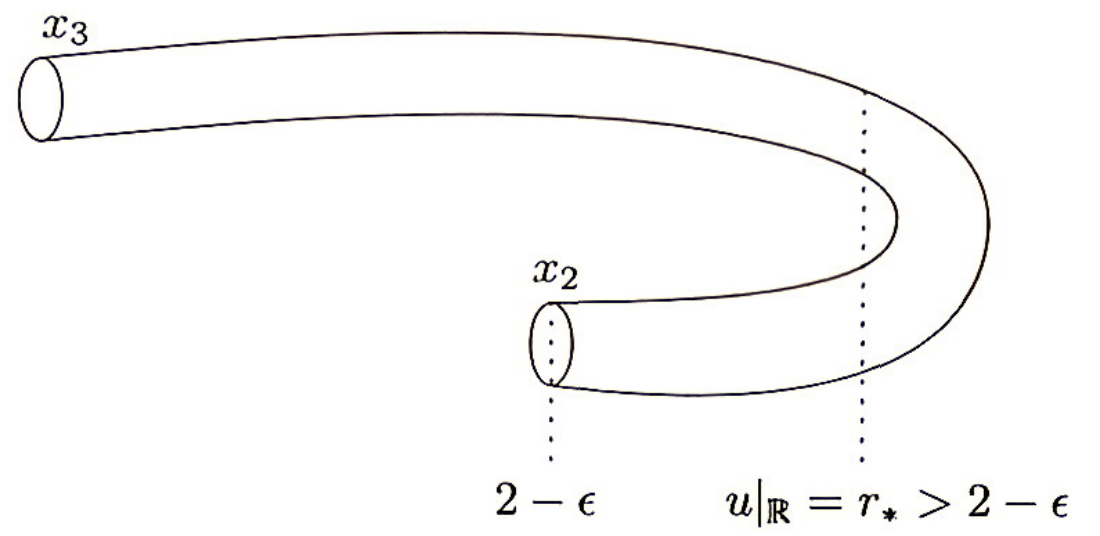
\includegraphics[width=0.62\linewidth]{figures/fig_p169_1.png}
  \caption*{图 6.9\quad $u$ 的图像（原书 p.161, Figure 6.9；PDF p.169）}
\end{figure}

然而，我们将证明一个多少相反的约束：若 Floer 轨道 $u$ 的两个渐近端都落在
$(0,r_\ast)\times\partial W$ 中（例如这里 $r_\ast$ 可以取得比 $2-\varepsilon$ 稍大，
其中 $x_2$ 位于 $r=2-\varepsilon$），则整条 $u$ 都落在 $(0,r_\ast)\times\partial W$
中。

假设不然，考虑区域
$S:=u^{-1}\bigl(\C^n\setminus(\{0\}\cup(-\infty,r_\ast)\times\partial W)\bigr)
\subset\R\times S^1$。关键在于考察 $u$ 的某种「能量」及其限制 $u|_S$。对任意 Floer
轨道 $u\colon\R\times S^1\to\C^n$，定义
\begin{align*}
  E(u)&:=\frac{1}{2}\int_0^1\int_{-\infty}^{\infty}
  \left(\left|\frac{\partial u}{\partial s}\right|^2
  +\left|\frac{\partial u}{\partial t}-X_H\right|^2\right)\dd s\,\dd t\\
  &=\frac{1}{2}\int_0^1\int_{-\infty}^{\infty}
  \omega\left(\frac{\partial u}{\partial s},J\left(\frac{\partial u}{\partial s}\right)\right)
  +\omega\left(\frac{\partial u}{\partial t}-X_H,
  J\left(\frac{\partial u}{\partial t}-X_H\right)\right)\dd s\,\dd t,
\end{align*}
因为 $|\cdot|^2=g_J(\cdot,\cdot)=\omega(\cdot,J\cdot)$。又因
$\frac{\partial u}{\partial t}-X_H=J\bigl(\frac{\partial u}{\partial s}\bigr)$，
我们有
\begin{align*}
  E(u)&=\int_0^1\int_{-\infty}^{\infty}
  \omega\left(\frac{\partial u}{\partial s},
  \frac{\partial u}{\partial t}-X_H\right)\dd s\,\dd t\\
  &=\int_{\R\times S^1}u^*\omega-\int_{\R\times S^1}(u^*\dd H)\wedge\dd t\\
  &=\int_{\R\times S^1}u^*\dd(r\alpha)-\int_{\R\times S^1}\dd(u^*H\wedge\dd t)\\
  &=\int_{\R\times S^1}\dd\bigl(u^*(r\alpha)-u^*H\dd t\bigr)\\
  &=\left(\int_{\{+\infty\}\times S^1}u^*(r\alpha)-u^*H\dd t\right)
  -\left(\int_{\{-\infty\}\times S^1}u^*(r\alpha)-u^*H\dd t\right)\\
  &=\bigl(r_+h'(r_+)-h(r_+)\bigr)-\bigl(r_-h'(r_-)-h(r_-)\bigr).
\end{align*}
于是由 (6.8)，我们知道
\begin{equation}\tag{6.13}
  E(u)=-\mathcal{A}_H\bigl((r_+,x_+)\bigr)+\mathcal{A}_H\bigl((r_-,x_-)\bigr)
  =-\mathcal{A}_H(x_3)+\mathcal{A}_H(x_2)\;(\ge0).
\end{equation}
考虑限制 $E(u|_S)$，按定义 $E(u|_S)\ge0$。然而，通过另一论证（见 [54] 中引理
2.2 的证明），可以证明 $E(u|_S)\le0$。详细的论证如下。

% >>> p170
首先，$u$ 的能量可以改写为
\begin{equation}\tag{6.14}
  E(u)=\frac{1}{2}\int_0^1\int_{-\infty}^{\infty}
  \bigl(|du-X_H\otimes\dd t|^2\bigr)\dd s\,\dd t,
\end{equation}
因为 $\langle X_H\otimes\dd t,du\rangle=\bigl\langle X_H,
\frac{\partial u}{\partial t}\bigr\rangle$。限制 $E(u|_S)$ 的定义是把 (6.14) 中的
积分区域 $\R\times S^1$ 换成区域 $S$。于是，用关于 $E(u)$ 的类似论证，可推出
\begin{align}
  E(u|_S)&=\int_S u^*\omega-(u^*\dd H)\wedge\dd t\notag\\
  &=\int_S\dd\bigl(u^*(r\alpha)-u^*H\dd t\bigr)\notag\\
  &=\int_{\partial S}\bigl(u^*(r\alpha)-u^*H\dd t\bigr)\notag\\
  &=\int_{\partial S}\bigl(r\alpha(\dd u)-u^*(r\alpha(X_H))\dd t\bigr)\notag\\
  &=\int_{\partial S}r\alpha\bigl(\dd u-X_H(u)\otimes\dd t\bigr).
  \tag{6.15}
\end{align}
这里第三行的等式来自 Stokes 定理。第四行的等式来自下述方程：
\[
  \int_{\partial S}u^*\bigl(r\alpha(X_H)-H\bigr)\dd t
  =\int_{\partial S}\mathcal{A}_H(r_\ast)\,\dd t
  =\int_S\mathcal{A}_H(r_\ast)\,\dd(\dd t)=0.
\]
记 $j$ 为 $S$ 上满足 $j\partial t=-\partial s$ 的复结构。注意我们可以把 Floer 方程
(5.21) 改写为
\[
  J\circ\bigl(\dd u-X_H(u)\otimes\dd t\bigr)
  =\bigl(\dd u-X_H(u)\otimes\dd t\bigr)\circ j,
\]
这与 $J$-全纯条件 $J\circ\dd u=\dd u\circ j$ 非常相似。于是 (6.15) 的最后一行可
写成
\begin{align*}
  \int_{\partial S}r\alpha\bigl(\dd u-X_H(u)\otimes\dd t\bigr)
  &=\int_{\partial S}r\alpha\Bigl(J\circ\bigl(\dd u-X_H(u)\otimes\dd t\bigr)\circ(-j)\Bigr)\\
  &=\int_{\partial S}r\,\dd r\circ\dd u\circ(-j)\le0,
\end{align*}
其中第一个等式来自 $r\alpha\circ J=r\,\dd r$（这由 3.3 节中 $J$ 的选取推出），以及
$\dd r(X_H)=\dd r(h'(r)R_\alpha)=0$。最后一个不等式来自下述论证：把 $\partial S$
写成两个 $S^1$ 的拷贝，并考虑 $S$ 的边界定向。$\partial S$ 上任意一点处的有序基
总由一个指向 $S$ 外部的向量与一个向量 $v=\pm\partial t$ 组成，其中 $v$ 的符号在 $S$
的两个边界分支 $S^1$ 上不同（见图 6.10）。在两种情形下，$jv=\pm j\partial t$ 总指向
$S$ 内部（因而指向 $(0,r_\ast)\times W$ 的外部），而 $\dd u(jv)$ 指向
$(0,r_\ast)\times W$ 的外部，使得 $\dd r\circ\dd u(jv)\ge0$。因此
$E(u|_S)=0$，这意味着 $u(S)\subset\{r_\ast\}\times\partial W$。矛盾。
\end{wproof}

% [Tutor Note: 易错预警——(6.15) 是「限制能量 = 边界积分」的典型计算，注意三处
% 符号与方向：(1) $\int_{\partial S}$ 的定向由 $S$ 诱导，$v=\pm\partial t$ 在两个
% 边界分支上取相反符号；(2) $r\alpha\circ J=r\,\dd r$ 只用到了 $J$ 把
% $\partial_r$ 方向送到 $R_\alpha$ 这一设计；(3) 最后的不等式方向依赖于 $jv$ 指向
% $S$ 内部，故 $\dd r\circ\dd u(-jv)$ 的符号为负。把这三点弄错会导致 $E(u|_S)$
% 的符号反转，从而无法得到矛盾。]

% >>> p171
\begin{figure}[htbp]
  \centering
  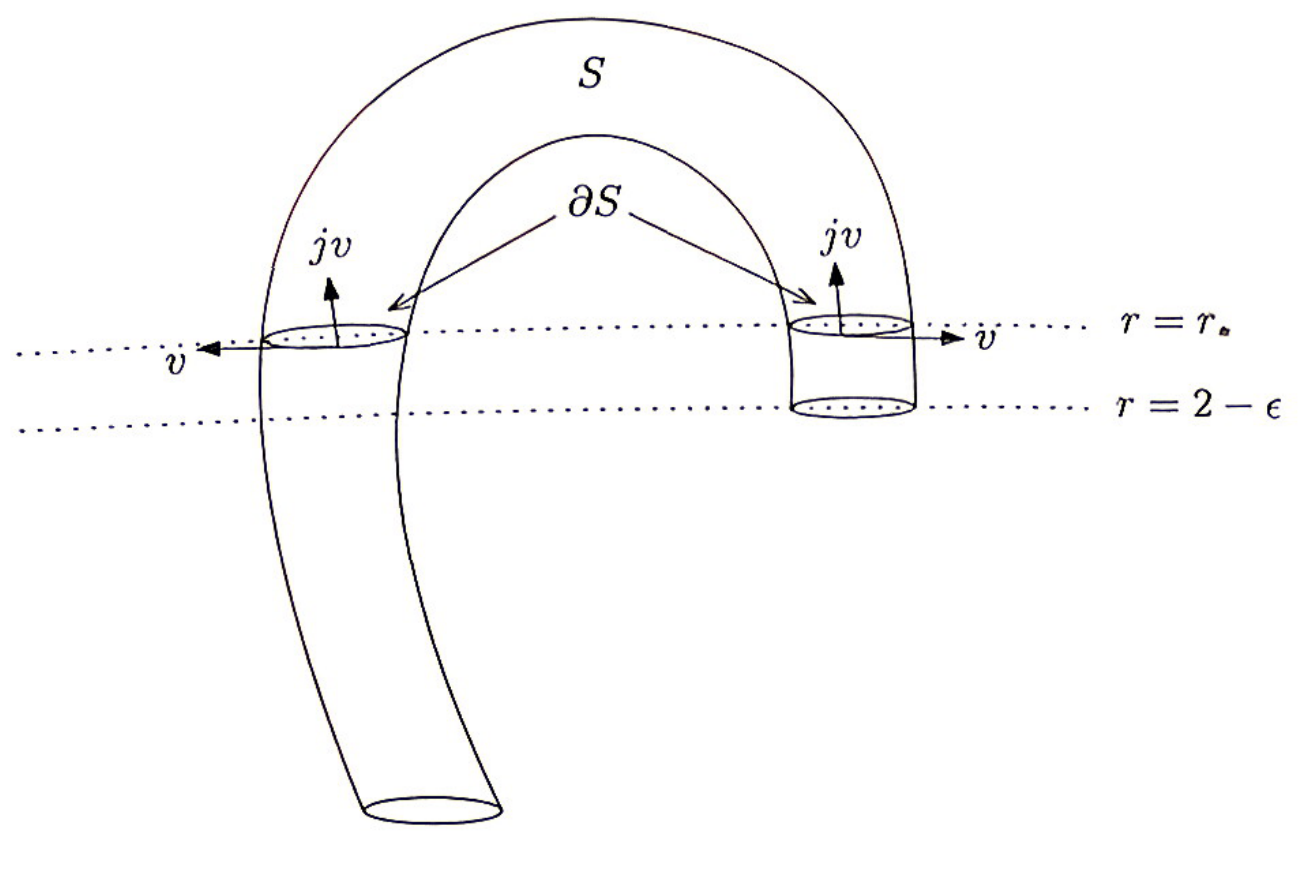
\includegraphics[width=0.66\linewidth]{figures/fig_p171_1.png}
  \caption*{图 6.10\quad $\partial S$ 上的向量 $v$ 与 $jv$
    （原书 p.163, Figure 6.10；PDF p.171）}
\end{figure}

\begin{wrem}{6.3.2}
  回忆 3.3 节中我们证明了：如 (6.10) 中的 $\R$-投影 $a(s,t)$ 是次调和的。因此，
  基于命题 6.3.1，也可以借助「次调和函数没有局部极大值」这一基本性质来证明断言
  6.3.1。
\end{wrem}

现在让我们回到本节开头所预告的刘维尔区域 $W\subset(\C^n,\dd\lambda_{\mathrm{std}})$
的辛同调，通常记作 $\mathrm{SH}_*(W)$。沿用 5.2 节引入的持续模语言，我们先定义
$\mathrm{SH}_*(W)$ 的过滤版本。

\begin{wdefn}{6.3.1}
  对 $a>0$，定义 $W$ 在水平 $a$ 处的\textbf{过滤辛同调}为
  \[
    \mathrm{SH}_*^{(a,\infty)}(W)
    :=\varprojlim_{H\in\mathcal{H}(W)}
    \mathrm{HF}_*^{(a,\infty)}(\C^n,\dd\lambda_{\mathrm{std}},H,J).
  \]
\end{wdefn}

这里，在分解 (6.7) 之下，$H(r,p)=h(r)$ 是图 6.11 所示的哈密顿函数，其中 $h(r)$
支撑在 $\{r\mid r\le1\}$ 中，且 $h(r)$ 在 $\{r\mid r\le1-\varepsilon\}$ 上是线性的，
其斜率\emph{不}落在 $\operatorname{Spec}(\partial W)$ 中；而
$\mathrm{HF}_*^{(a,\infty)}(\C^n,\dd\lambda_{\mathrm{std}},H,J)$ 是由作用量
$\mathcal{A}_H>a$ 的闭哈密顿轨道生成的哈密顿 Floer 同调（见 5.4 节与 (6.2)）。
这类函数的全体记作 $\mathcal{H}(W)$。

\begin{figure}[htbp]
  \centering
  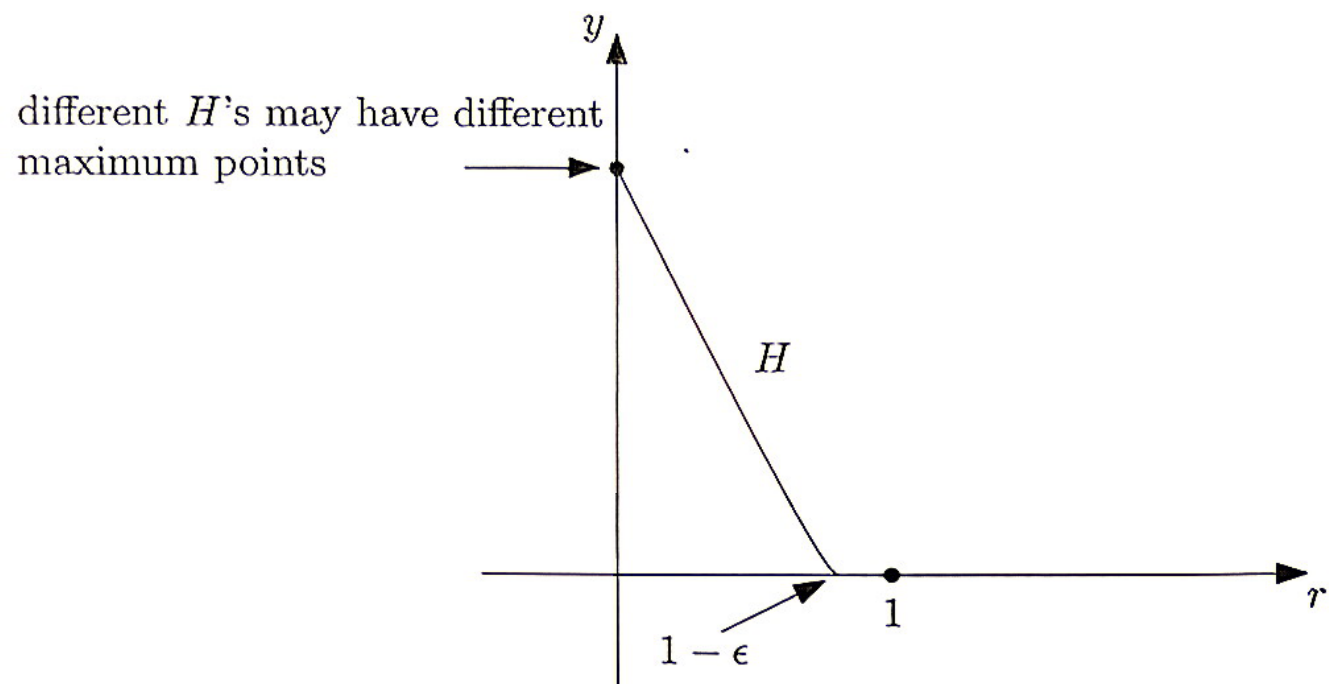
\includegraphics[width=0.5\linewidth]{figures/fig_p172_1.png}
  \caption*{图 6.11\quad $\mathcal{H}(W)$ 中的函数
    （原书 p.164, Figure 6.11；PDF p.172）}
\end{figure}



作为消化定义 6.3.1 的第一步，我们来回顾逆向极限 $\varprojlim$。给定指标集
$(I,\le)$，它偏序且向下定向，意指对任意 $i,j\in I$，存在 $k\in I$ 使得 $k\le i$
且 $k\le j$；$(I,\le)$ 上的一个 $\mathbf{k}$-模\textbf{逆向系统}是下述数据
\[
  (A,\sigma):=\bigl(\{A_i\}_{i\in I},
  \{\sigma_{ij}\colon A_i\to A_j\}_{i\ge j\in I}\bigr),
\]
其中每个 $A_i$ 是 $\mathbf{k}$-模，且对任意 $i\ge j\ge k$（$i,j,k\in I$）有
$\sigma_{ik}=\sigma_{jk}\circ\sigma_{ij}$ 与 $\sigma_{ii}=\mathbf{1}_{A_i}$。

% >>> p172
于是 $(A,\sigma)$ 的\textbf{逆向极限}（inverse limit）定义为
\begin{equation}\tag{6.16}
  \varprojlim_{i\in I}A
  :=\left\{(x_i)_{i\in I}\in\prod_{i\in I}A_i
  \;\middle|\;\sigma_{ij}(x_i)=x_j\right\}.
\end{equation}
注意我们有投影映射 $\pi_i\colon\varprojlim_{i\in I}A\to A_i$，满足：对任意
$i\le j$，有 $\sigma_{ij}\circ\pi_i=\pi_j$。

遗憾的是，这个定义对计算 $\varprojlim_{i\in I}A$ 并无帮助。下面是一个常用于计算的
有用事实。

\whead{事实}{6.3.1（[29] 中的引理 4.7.1）}设 $(A,\sigma)$ 是一个逆向系统。假设它
允许一个\textbf{向下穷竭序列} $\{A_{i_v}\}_v$，其意义如下：
\begin{enumerate}[label=(\roman*)]
  \item 对任意 $i\in I$，存在 $i_v\le i$；
  \item 对任意 $i_{v+1}\le i_v$，映射
        $\sigma_{i_{v+1}i_v}\colon A_{i_{v+1}}\to A_{i_v}$ 是同构。
\end{enumerate}
则投影 $\pi_{i_v}\colon\varprojlim A\to A_{i_v}$ 是同构。特别地，对任意 $i_v$ 有
$\varprojlim A\cong A_{i_v}$。

\begin{wexam}{6.3.4}
  考虑定义 6.3.1 的框架中记作 $\mathcal{H}(W)$ 的哈密顿函数空间
  $H(r,p)=h(r)$。在 $\mathcal{H}(W)$ 上如下定义偏序 $\preccurlyeq$：
  \begin{equation}\tag{6.17}
    H\preccurlyeq G\quad\text{当且仅当}\quad
    H(r,p)\ge G(r,p)\ \text{对任意 }(r,p)\in\C^n.
  \end{equation}
  由 7.1 节关于 Floer 延拓映射的讨论，对 $\mathcal{H}(W)$ 中任意 $H\preccurlyeq G$，
  存在良定义的映射
  $\sigma_{H,G}\colon\mathrm{HF}_*^{(a,\infty)}(\C^n,\dd\lambda_{\mathrm{std}},H,J)
  \to\mathrm{HF}_*^{(a,\infty)}(\C^n,\dd\lambda_{\mathrm{std}},G,J)$，但它不必是
  同构！重要的是，如我们已经看到的，$\sigma_{H,G}$ 保持作用量 $a$，其意义是：作用量
  落在作用量窗口 $(a,\infty)$ 中的闭哈密顿轨道将被映到作用量同样落在 $(a,\infty)$
  中的轨道。事实上，上述数据对每个固定的 $a>0$ 组合成一个逆向系统
  \begin{equation}\tag{6.18}
    \bigl(\{\mathrm{HF}_*^{(a,\infty)}(H)\}_{H\in\mathcal{H}(W)},
    \{\sigma_{H,G}\colon\mathrm{HF}_*^{(a,\infty)}(H)\to
    \mathrm{HF}_*^{(a,\infty)}(G)\}_{H\preccurlyeq G\in\mathcal{H}(W)}\bigr).
  \end{equation}

  \hfill$//$
\end{wexam}

% >>> p173
计算这个逆向系统的逆向极限完全由 $\sigma_{H,G}$ 决定，但一般而言这些 $\sigma_{H,G}$
的精确公式是未知的。幸运的是，在某些特殊情形，比如取一列哈密顿函数
$H_i^\varepsilon(r,p)=h_i^\varepsilon(r)\in\mathcal{H}(W)$（$i\in\N$），其中
\begin{equation}\tag{6.19}
  h_i^\varepsilon(0)=a+\varepsilon\cdot i
  \qquad\text{对任意固定的（小）}\varepsilon>0,
\end{equation}
则 [29] 中的命题 4.5.1 蕴含 $\sigma_{H_i^\varepsilon,H_j^\varepsilon}$ 全是同构。
因此，事实 6.3.1 蕴含下述重要结果，它把一个逆向极限转化为单个哈密顿函数的计算：
\begin{equation}\tag{6.20}
  \mathrm{SH}_*^{(a,\infty)}(W)\cong\mathrm{HF}_*^{(a,\infty)}(H_a),
\end{equation}
其中哈密顿函数 $H_a(r,p)=h_1^\varepsilon(r)$，$\varepsilon>0$ 取某个优选的小值，
并使得 $H_a(0)$ 略高于值 $a$。

考虑作用量窗口 $(a,+\infty)$ 与图 6.11 那样的哈密顿函数的过滤辛同调，其优点在于：
当 $\max_{\C^n}H_a=H_a(0)$ 非常接近 $a$ 时（通过把 (6.19) 中的 $\varepsilon$ 取得
充分小），$\mathcal{A}_H$ 只有一个临界点——即位于 $0$ 的常值闭哈密顿轨道——的
作用量落在 $(a,\infty)$ 中，而其余来自 $\partial W$ 在 $r=1-\varepsilon$ 附近的非
常值闭 Reeb 轨道的轨道，其作用量严格小于 $a$（见图 6.12）。因此，由 (6.20)，我们
可以显式地算出 $\mathrm{SH}_*^{(a,\infty)}(W)$：
\begin{equation}\tag{6.21}
  \mathrm{SH}_*^{(a,\infty)}(W)
  =(0\in\C^n\ \text{处的常值闭哈密顿轨道}).
\end{equation}
唯一未确定的信息是这个单一生成元的次数（或指标），它由定义 5.5.1 中的
Conley--Zehnder 指标给出。由例 5.5.7 的计算经验，作用量窗口 $(a,\infty)$ 中的参数
$a$ 越大（从而相应的轮廓 $h(r)$ 在 $0$ 附近的斜率越负），该次数的绝对值就越高。

\begin{figure}[htbp]
  \centering
  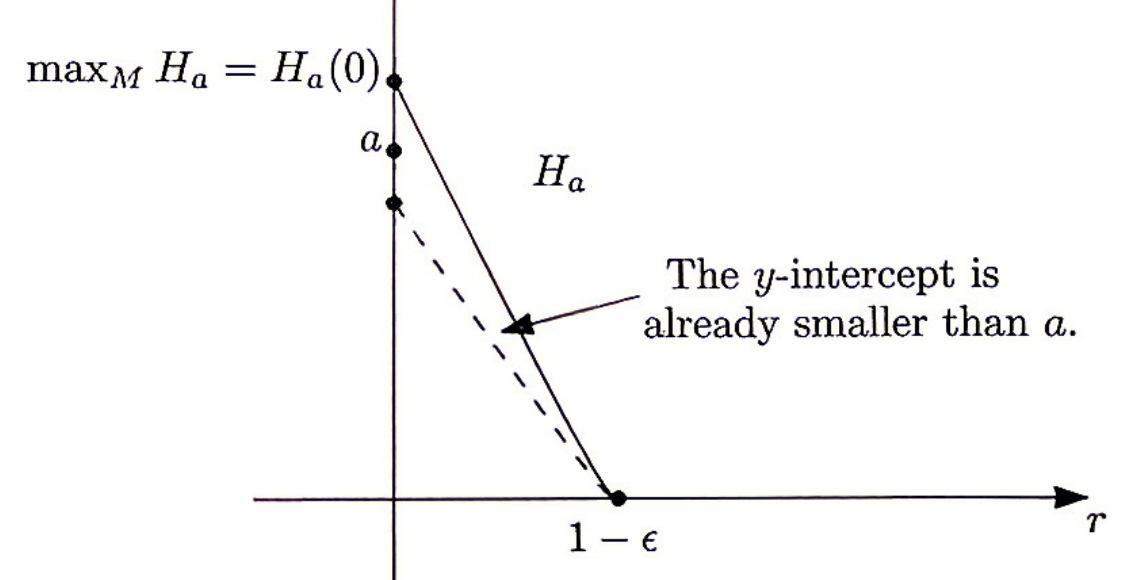
\includegraphics[width=0.5\linewidth]{figures/fig_p173_1.png}
  \caption*{图 6.12\quad 值 $\max H_a$ 非常接近 $a$
    （原书 p.165, Figure 6.12；PDF p.173）}
\end{figure}



% [Tutor Note: 易错预警——(6.21) 的等式应理解为「同调群作为 $\Z_2$-向量空间由单个
% 生成元张成」，即 $\mathrm{SH}_*^{(a,\infty)}(W)\cong\Z_2$ 集中在某个次数上；
% 而这个次数（Conley--Zehnder 指标）恰是 (6.25) 中辛同调容量的关键：容量取的是
% 「最低次数的区间的最左端点」。另注意 (6.20) 的下标 $H_a$ 指 $h_1^\varepsilon$，
% 而非 $h_a$；$\varepsilon$ 的选取与 $a$ 有关。]

% >>> p174
\begin{figure}[htbp]
  \centering
  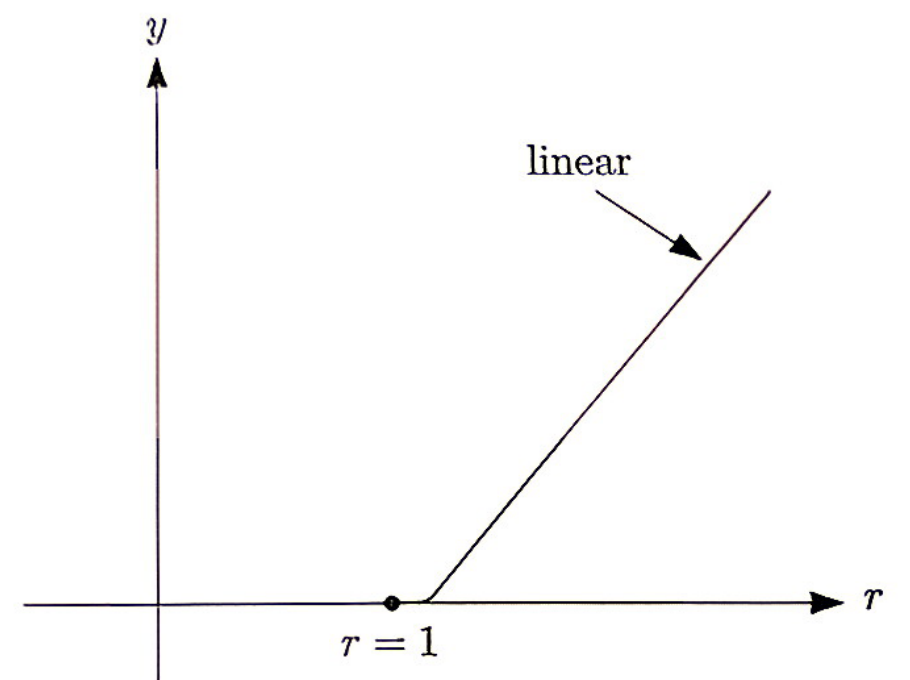
\includegraphics[width=0.6\linewidth]{figures/fig_p174_1.png}
  \caption*{图 6.13\quad 另一类哈密顿函数（原书 p.166, Figure 6.13；PDF p.174）}
\end{figure}

\begin{wrem}{6.3.3}
  除上述族 $\mathcal{H}(W)$ 之外，我们还可以选取其他族的哈密顿函数，用类似方式
  构造同调理论。例如，若 $H_a$ 形如图 6.13——一种与图 6.11 所示函数多少相反的
  哈密顿函数。由此得到的辛同调理论最早由 C.~Viterbo 在 [234] 中发明。
\end{wrem}

现在，对任意刘维尔区域 $W\subset(\C^n,\dd\lambda_{\mathrm{std}})$，我们构造一个
（如定义 5.2.1 那样以 $\R$ 为参数的）持续 $\Z_2$-模。对任意 $r\in\R$，考虑
$\mathrm{SH}_*^{(e^r,\infty)}(W)$，则所需的持续 $\Z_2$-模由下述数据组成：
\begin{equation}\tag{6.22}
  \mathbb{V}_W=\bigl(\{V_t:=\mathrm{SH}_*^{(e^r,\infty)}(W)\}_{r\in\R},
  \{\iota_{r,s}\colon\mathrm{SH}_*^{(e^r,\infty)}(W)\to
  \mathrm{SH}_*^{(e^s,\infty)}(W)\}_{r\le s}\bigr),
\end{equation}
其中 $\iota_{r,s}$ 由标准态射
$\mathrm{HF}_*^{(e^r,\infty)}(H)\to\mathrm{HF}_*^{(e^s,\infty)}(H)$（当 $r\le s$）
诱导。

\begin{wexer}{6.3.1}
  写出 $\iota_{r,s}$ 的定义。（提示：使用逆向极限的泛性质。）
\end{wexer}

下述定义从 (6.22) 的信息中萃取而来。

\begin{wdefn}{6.3.2}
  设 $W\subset(\C^n,\dd\lambda_{\mathrm{std}})$ 是刘维尔区域。则定义 $W$ 的
  \textbf{辛同调}为
  \[
    \mathrm{SH}_*(W):=\lim_{r\to\infty}V_r,
  \]
  其中 $V_r$ 来自 (6.22)，而正向极限（见定义 10.2.5）沿参数 $r\in\R$ 取。
\end{wdefn}

通过反思上述讨论，不难得出结论：对刘维尔区域
$W\subset(\C^n,\dd\lambda_{\mathrm{std}})$，对任意次数 $*$ 都有
$\mathrm{SH}_*(W)=0$。然而相反地，下述例子表明 (6.22) 中的持续 $\Z_2$-模
$\mathbb{V}_W$ 极不平凡。

% >>> p175
\begin{wexam}{6.3.5}
  设 $W=E(1,N,\cdots,N)$ 是 $2n$ 维椭球，其中 $N\gg1$ 且 $N$ 是无理数。对 (6.22)
  中的持续 $\Z_2$-模 $\mathbb{V}_W$，限制在次数 1 上时，有
  \[
    V_r=\Z_2\qquad\text{对 } r\in(-\infty,0],
  \]
  这意味着 $\mathbb{V}_W$ 在次数 $1$ 上的条形码为
  $\mathbb{B}(\mathbb{V}_W)|_{*=1}=\{(-\infty,0]\}$。限制在次数 3 上时，有
  \[
    V_r=\Z_2\qquad\text{对 } r\in(0,\ln2].
  \]
  注意 $\mathbb{B}(\mathbb{V}_W)$ 的条形码中前几个区间形如
  \[
    \{(-\infty,0],\ (0,\ln2],\ (\ln2,\ln3],\ \cdots\},
  \]
  其中次数依次为 $1,3,5,\cdots$。它们都来自作用量等于 $1$ 的简单闭 Reeb 轨道的
  迭代。当迭代的次数足够高时，另一条作用量等于 $N$ 的简单闭 Reeb 轨道将发挥作用，
  并可能与其他轨道相互作用。类似地，若 $W=B^{2n}(r)$，可以得出结论：持续
  $\Z_2$-模 $\mathbb{V}_W$ 的条形码满足
  $\mathbb{B}(\mathbb{V}_W)|_{*=1}=\{(-\infty,\ln r]\}$。\hfill$//$
\end{wexam}

% [Tutor Note: 原文疑误——例 6.3.5 中先称「限制在次数 1 上」得到
% $V_r=\Z_2\ (r\in(-\infty,0])$，紧接着却说「$\mathbb{V}_W$ 在次数 0 上的
% 条形码」，而紧接着的记号 $\mathbb{B}(\mathbb{V}_W)|_{*=1}$ 与下文「次数依次为
% $1,3,5,\cdots$」都表明应为次数 1。据此判断「degree 0」是「degree 1」的笔误。
% 已记入 review_ch06.md。另注意：$V_r=\Z_2$ 对 $r\in(-\infty,0]$ 成立，等价于
% 条形码中出现左端点为 $-\infty$、右端点为 $0$ 的条，即 $(-\infty,0]$。]

与定义 6.3.2 类似，可以对任意（非退化的）刘维尔区域 $W$ 定义辛同调
$\mathrm{SH}_*(W)$，其中 $\C^n$ 由其完形 $\widehat{W}$ 代替（见例 3.2.4 正上方的
讨论）。一个典型的例子是黎曼（或 Finsler）流形 $(Q,g)$ 的单位余盘丛 $D_g^*Q$
（在 (3.11) 中定义），此时完形就是整个余切丛 $T^*Q$。与
$W\subset(\C^n,\dd\lambda_{\mathrm{std}})$ 的 $\mathrm{SH}_*(W)$（如上所述恒等于
零）本质不同的是，$\mathrm{SH}_*(D_g^*Q)$（在域 $\Z_2$ 上）永不消失。下述结果是
辛几何中最有用的结果之一，我们直接陈述其过滤版本。

\begin{wthm}{6.3.1（Viterbo 同构 [4, 5, 6, 194, 234, 240]）}
  给定 Finsler 流形 $(Q,g)$，对任意 $a>0$ 存在同构
  \begin{equation}\tag{6.23}
    \mathrm{SH}_*^{(a,\infty)}(D_g^*Q;\Z_2)
    \cong H_*\bigl(\Lambda^{\frac{a^2}{2}}Q;\Z_2\bigr),
  \end{equation}
  其中
  $\Lambda^{\frac{a^2}{2}}Q:=\bigl\{\gamma\colon S^1\to Q\;\big|\;
  E_g(\gamma)<\frac{a^2}{2}\bigr\}$，而 $E_g(\gamma)$ 表示 $\gamma$ 的能量。
\end{wthm}

(6.23) 的右端是经典的（过滤）圈空间同调，它由 $(Q,g)$ 上的闭测地线生成。因此，
定理 6.3.1 中的同构提供了用辛方法研究闭测地线问题的机会。该方向的应用见
[211]。

% [Tutor Note: 含糊点拨——Viterbo 同构把「辛同调（动力学不变量）」与「圈空间同调
% （拓扑不变量）」等同起来，是辛几何与拓扑之间的桥梁。注意 (6.23) 中过滤参数
% $a$ 与能量的关系是 $E<\frac{a^2}{2}$ 而不是 $E<a$ 或 $E<a^2$：若把 $a$ 理解为
% 长度（作用量 $=$ 长度），则能量 $=\frac12\int|\dot\gamma|^2=\frac12(\text{长度})^2$，
% 这正是因子 $\frac12$ 的来源；$D_g^*Q$ 中的余向量范数取 $g$ 的对偶范数。
% 该同构的证明用到了 Floer 理论中的「作用量—能量」对应与有限型条件，建议参考
% Viterbo, \emph{Funct. Anal.} 1999 或 Abbondandolo--Schwarz 的综述。]
